
\begin{figure}[h]%deepNN
\centering
\scalebox{0.9}{
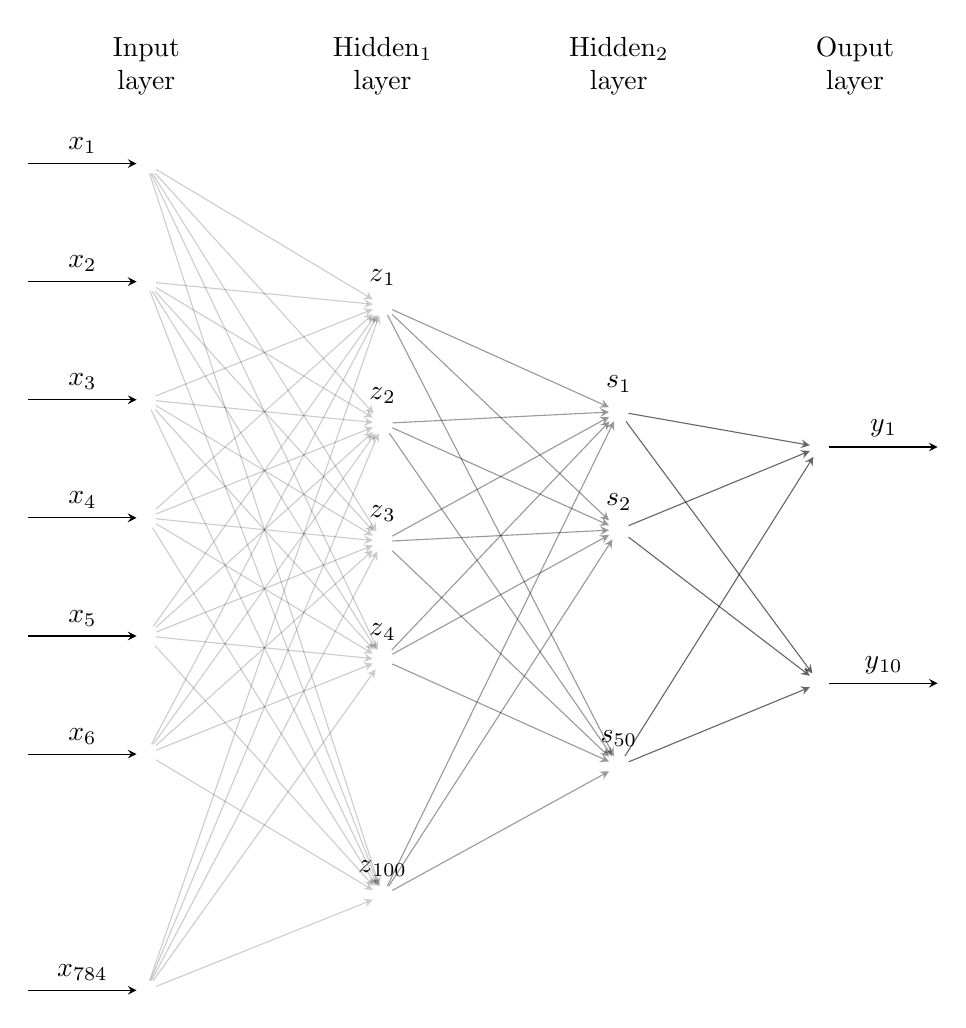
\begin{tikzpicture}[x=1.5cm, y=1.5cm, >=stealth]
\foreach \m/\l [count=\y] in {1,2,3,4,5,6,missingl,7}
  \node [every neuron/.try, neuron \m/.try] (input-\m) at (0,2.5-\y) {};
\foreach \m [count=\y] in {1,2,3,4,missingl,5}
  \node [every neuron/.try, neuron \m/.try ] (hidde-\m) at (2,2-\y-0.7) {};
\foreach \m [count=\y] in {1,2,missingl,3}
  \node [every neuron/.try, neuron \m/.try ] (hidden-\m) at (4,1.5-\y-1.1) {};
  \foreach \m [count=\y] in {1,missingl,2}
  \node [every neuron/.try, neuron \m/.try ] (output-\m) at (5.7,1.5-\y-1.4) {};
\foreach \l [count=\i] in {1,2,3,4,5,6,{784}}
  \draw [<-] (input-\i) -- ++(-1,0)
    node [above, midway] {$x\textsubscript{\l}$};
\foreach \l [count=\i] in {1,2,3,4,100}
  \node [above] at (hidde-\i.north) {$z\textsubscript{\l}$};
\foreach \l [count=\i] in {1,2,50}
  \node [above] at (hidden-\i.north) {$s\textsubscript{\l}$};
\foreach \l [count=\i] in {1,10}
  \draw [->] (output-\i) -- ++(1,0)
    node [above, midway] {$y\textsubscript{\l}$};
\foreach \i in {1,...,7}
  \foreach \j in {1,...,5}
    \draw [opacity=0.2][->] (input-\i) -- (hidde-\j);
\foreach \i in {1,...,5}
  \foreach \j in {1,...,3}
    \draw [opacity=0.4][->] (hidde-\i) -- (hidden-\j);
\foreach \i in {1,...,3}
  \foreach \j in {1,...,2}
    \draw [opacity=0.6][->] (hidden-\i) -- (output-\j);
\foreach \l [count=\x from 0] in {Input, Hidden\textsubscript{1}, Hidden\textsubscript{2}, Ouput}
  \node [align=center, above] at (\x*2,2) {\l \\ layer};
\end{tikzpicture}}
\caption{Deep Neural Network}
\label{deepNN}
\end{figure}

